\chapter{Application Development Plan}

A visualization for the plan for this project can be seen in the Gannt chart in figure \ref{fig:gannt}
\begin{figure}
	\caption[Gannt Chart of the Project]{Gannt chart showing the project's planned process over the academic year.}
	\label{fig:gannt}
	\begin{center}
	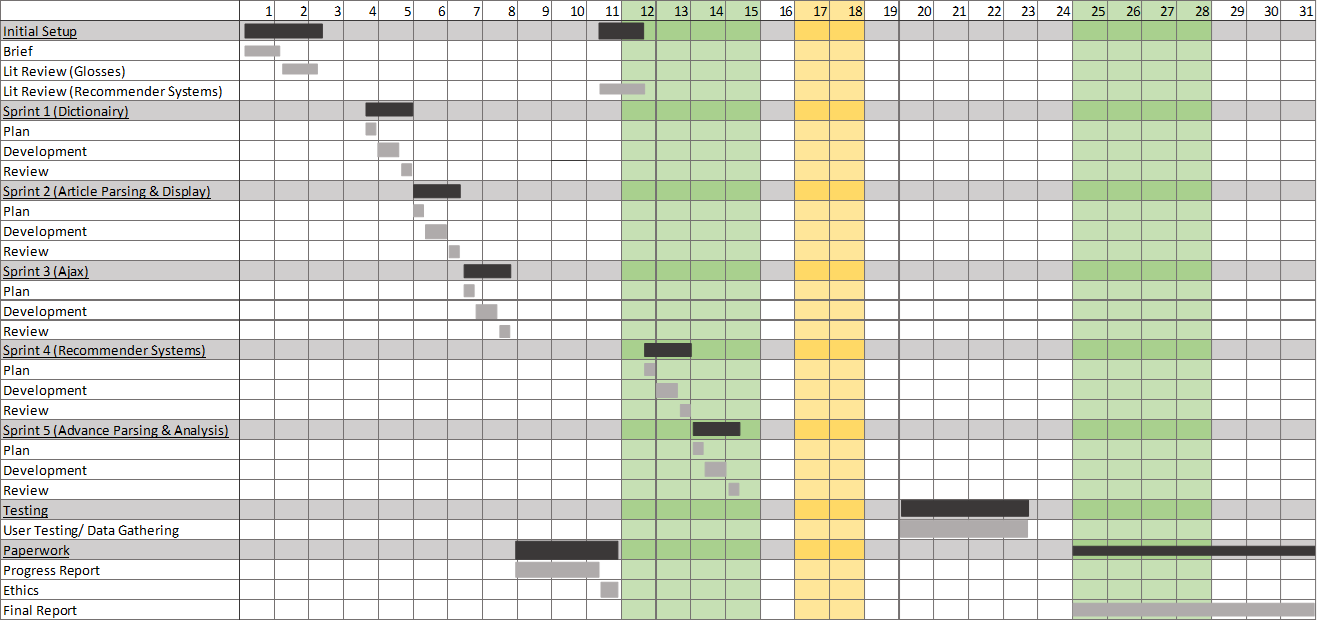
\includegraphics[width=\textwidth]{Graphics/Gannt}
	\end{center}
\end{figure} 

\section{Readings and Research}

The plan details that reading was to be divided into two parts, reading about glosses and reading about difficulty rating systems. With the reading about difficulty rating systems being done after the gloss was developed. This was done as the difficulty rating system was not part of the minimum viable project, so the reading about it could be left until after the development of the minimum viable project was complete. The vast majority of this reading was academic, looking into the effectiveness of various glosses and methods of rating the difficulty of articles.

Other reading was done during the planning stage of each sprint, this reading was more technical and was about researching and deciding upon the technologies that were to be used for that sprint. Once a technology had been decided upon, there was some time spent on learning how to integrate it with project.


\section{Development}

The application was developed using AGILE methods. these methods were used as they allowed the developer to have regular meetings with the project supervisor, discussing the progress made, what was left to be done whether or not it was achievable.

\section{Testing}

Three types of testing were done on the application. Unit testing was during the development of sprint one, to ensure that the application was interacting with the dictionary API correctly, making sure that the correct translations of various words were found. 

functional testing was during the development of the rest of the application, the developer would use the application, testing whether or not the feature they were currently implementing was working as planned.

Finally, user testing was done once all six sprints were completed, it consisted on the user using the application to read three articles, and then filling out a feed back survey about their experiences with it. In addition, the user's use of the application was tracked, seeing what words they requested and what articles they read. Ethics approval for this test was obtained from the ECS ethics board. 